\documentclass[twocolumn]{article}
\usepackage{fullpage}
\usepackage{mathpazo}
\usepackage{hyperref}
\usepackage{cite}
\usepackage{graphicx}
\usepackage{verbatim}

\begin{document}
  
  \title{GPU Project Final Report: Accelerated RC4 Stream Cipher}
  \author{Guy Dickinson (guy.dickinson@nyu.edu) \& William Ward, (wwward@nyu.edu)}
  \maketitle
  
  \section{Introduction}
  The RC4\footnote{RC4 remains a trademark of RSA; RC4 is alternately known as ARCFOUR but referred to here as RC4 for clarity.} cipher is a widely used stream cipher found in many common applications, from WEP/TKIP \cite[p. 171]{cisco-netsec} to OpenSSL \cite{openssl}. It is a stream cipher with a particularly simple encipher/decipher operation; the actual mutation of plaintext to ciphertext is a simple bitwise XOR operation against a keystream generated from a relatively straightforward state machine initialized with a secret key of arbitrary length.
  
  The specification for RC4 has never officially been released by its corporate owner, RSA, although its creator, Ron Rivest, has tacitly acknowledged veracity of the public implementations of RSA by linking to the Wikipedia page for RC4 in his course notes at MIT.\cite{rivest-notes}
  
  Previous work in this area \cite{5276924} was largely been limited to a proof-of-concept implementation which encrypted and decrypted static files on-disk. This gave the authors the luxury of knowing exactly how much data is to be encrypted before the program is run. Such is not the life a stream cipher in the field; a stream cipher must be able to take arbitrary amounts of data at any given moment and efficiently process it. Our implementation efficiently streams data to and from the GPU making use of CUDA's multi-stream instruction architecture. 
  
  \section{Design}
  
  Our RC4 implementation has two major operations and three major components. The components are:
  
  \begin{itemize}
    \item An array, $A_t$ of arbitrary length $l$  bytes containing the target data to be encrypted or decrypted.
    \item A second array $A_k$, also of length $l$ bytes, containing the keystream with which the data is to be encrypted.
    \item A data structure $M$ which represents the current state of the keystream generator. That data structure contains:
    \begin{itemize}
      \item A an array of all 256 possible bytes (that is to say, all possible 8-bit binary combinations, $2^8=256$ in total).
      \item Two pointers, $i$ and $j$ which are used to exchange bytes in the permutation.
    \end{itemize}
  \end{itemize}
  
  The operations are:
  
  \begin{itemize}
    \item Initialization of the RC4 state.
    \item Encryption/decryption of data.
  \end{itemize}
  
  Initialization is performed only once per run of the RC4 algorithm and takes negligible time. Encryption/decryption is performed with the simple operation $A_k \oplus A_t$
  
  RC4 presents an interesting challenge from a parallelization perspective: although the actual bit-flipping operation can be parallelized very easily, generating the keystream is an inherently parallel operation. That is to say, the operation of calculating byte $n$ of the keystream explicitly requires byte $n-1$ to perform.
  
  Because generating the keystream is so inherently parallel, trying to contort the GPU into performing this task made no sense; the key-scheduler and its operation remains on the CPU. All encryption and decryption is done on the GPU.
  
  Instead of reading from a file using C's \texttt{fread()} functions, we take input from the standard input stream, to simulate an environment where data arrives one byte at a time and the total length of the data is not known; EOF may be reached at any time.
    
  \subsection{Partitioning}
  Partitioning of data is somewhat trivial for RC4 since the structures are simply one-dimensional arrays of a known length:
  
  Data is captured into a buffer of fixed length $l$, specified at run-time. During testing, we used a buffer size of 512, but this can be increased arbitrarily. When the buffer is full, it is flushed and encrypted against a chunk of keystream also of length $l$.
  
  
  \subsection{GPU Grid Geometry}
  
  
  \section{Optimizations}
  \subsection{Buffering}
  During our initial proof-of-concept work, we simply read one byte at a time, generated one byte of keystream, sent both to the GPU, then recovered the result. This is slow and inefficient because keystream generation and memory copying are blocking, so for every byte of input data, we make three blocking calls, completely obviating any benefit of GPU acceleration--and significantly slowing the serial implementation as well.
  
  Instead of calculating the key for every byte, we wait until an input buffer is full, calculate the keystream for that buffer, then send the buffer and key to the GPU for processing. Further optimization could also be found in asynchronously generating the keystream while the buffer is filling, however, this would require the use of \texttt{pthreads} on the CPU which we found to be beyond the scope of this project.
  
  \subsection{Asynchronous GPU Transfer}
  
  We further optimized the CPU/GPU transfers by using a multi-stream transfer/compute interleaving technique\cite{gpu-conf}. We set up two streams, $S_1$ and $S_2$. At each `cycle', we:
  
  \begin{itemize}
    \item Asynchronously start the transfer of data to the GPU from $A_t$ and $A_k$ on the CPU using stream $S_1$.
    \item Asynchronously recover encrypted data from $A_t$ on the GPU using stream $S_1$.
    \item Asynchronously invoke a kernel which encrypts the data already on the GPU using stream $S_2$.
    \item Capture $l$ bytes of fresh material into a buffer on the host.
  \end{itemize}
  
  We then wait for both streams to complete, then output the data recovered from the GPU.
  
  This allows the two memory transfers, kernel invocation, and fresh material to happen in an asynchronous, interleaved manner, which hides the substantial latency inherent in transferring data to and from the GPU via the PCIe bus.

  
  \section{Experimental Setup}
  
  We tested this setup on a Tesla T10 Processor with CUDA compute capability 1.3. The Tesla T10 sports a total of 240 CUDA cores, maximally allowing 512 threads per block. Because we took extra steps to hide the latency in the CPU-GPU transfers, we simply used the UNIX \texttt{time} utility to measure the total execution time of our programs.
  
  \section{Results}
  
  %\begin{comment}
  \begin{table}
  \tiny
  \begin{tabular}{| c | c | c | c | c | c |}
. & SerialCPU & Par512 & ParInt512 & Par16.7M & ParInt16.7M \\ \hline
SerialCPU & 100.00\% & 217.73\% & 275.18\% & 71.11\% & 69.51\% \\ \hline
Par512 & 45.93\% & 100.00\% & 126.39\% & 32.66\% & 31.93\% \\ \hline
ParInt512 & 36.34\% & 79.12\% & 100.00\% & 25.84\% & 25.26\% \\ \hline
Par16.7M & 140.62\% & 306.17\% & 386.96\% & 100.00\% & 97.75\% \\ \hline
ParInt16.7M & 143.86\% & 313.23\% & 395.87\% & 102.30\% & 100.00\% \\ \hline
  \end{tabular}
  \end{table}
  %\end{comment}
  
  \includegraphics[scale=0.25]{gpuruntimes.eps} 

  \section{Conclusions}
   todo: what is the limiting factor of the 16.7M buffersize?

  \section{Additional Notes}
  All experimental code may be found at \url{https://github.com/gdickinson/gpuclass}.
  
  \bibliography{final}{}
  \bibliographystyle{plain}
  
\end{document}